% Source: Weinberg GR, physical PDF pp. 461 and 463 (printed p. 439,
% repeated in the local scan).
% Coverage: Figure 14.10, M87 at four polarization orientations.
% Status: source photographs extracted at source resolution; source-reviewed and compile-clean.
% Uncertainties: none.

\begingroup
\renewcommand{\thefigure}{14.10}
\begin{figure}[htbp]
  \centering
  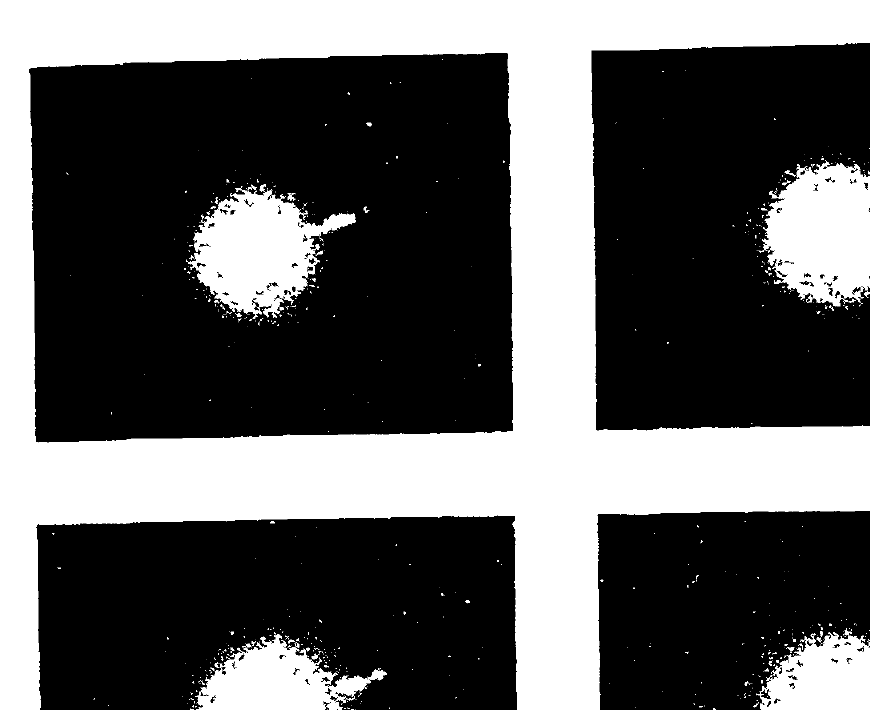
\includegraphics[width=0.82\textwidth]{figures/chapter14/fig14-10.png}
  \caption{The giant elliptical galaxy M87 (NGC 4486) in the Virgo cluster,
  for four different directions of polarization. These photographs, taken
  with the 200-in.\ telescope at Mt.\ Palomar, are underexposed in order to
  reveal the galactic nucleus and the remarkable ``jet.'' (Courtesy Mt.\
  Wilson and Mt.\ Palomar observatories.)}
  \label{fig:14.10}
\end{figure}
\endgroup
